\begin{figure}[h!]
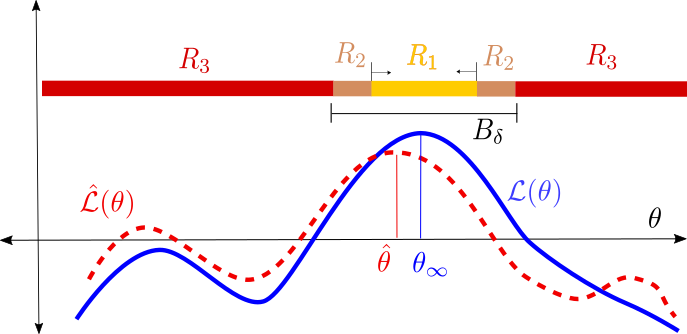
\includegraphics[width=\textwidth]{static_figures/BCLT_illustration.png}
\caption{Visual illustration of the proof technique.  As $N$ increases,
$\likhat(\theta) \rightarrow \lik(\theta)$
uniformly within $\thetaball{\delta}$, $\likhat(\theta)$ remains
bounded away from $\likhat(\thetatrue)$ outside of $\thetaball{\delta}$,
and the region $R_1$ that matters for the posterior shrinks at
a rate slightly slower than $1/\sqrt{N}$.}
\figlabel{proof_technique}
\end{figure}
